\documentclass[draft]{article}
\usepackage[T1]{fontenc}
\usepackage{microtype}
\usepackage{xcolor}
\usepackage{graphicx}


\def\useful#1{\textcolor{teal}{#1}}
\def\text{Lorem ipsum dolor sit amet, consectetuer adipiscing elit.%
Ut purus elit,vestib\-ulum ut, placerat ac, adipiscing vitae, felis. Curabitur dictum gravida%
mauris.}


\begin{document}
\section{The primitive \texttt{list}}
\subsection{list}
All the vertical length is rubber, all the horizontal length is rigid.

\newcounter{Bean}
\begin{list}
  {<Prefix>--\Roman{Bean}}
  {\usecounter{Bean}
  \setlength{\leftmargin}{0pt}
  \setlength{\rightmargin}{10em}
  \setlength{\labelsep}{\dimexpr.5em}
  \setlength{\labelwidth}{50em}
  % \setlength{\labelsep}{2ex}
  \setlength{\itemindent}{\dimexpr 2ex+0ex}
  \setlength{\parsep}{3em plus .5em minus 1.5em}
  }
  \item[\textbf{Label Label a}] \useful{Use the default labelsep, it turns out that the label has stick in the item content. 
    The Length is: labelsep=\the\labelsep. Then we set the length `labelsep'.}
    \setlength{\labelsep}{2ex}
  \item[\texttt{\textbackslash str\_map\_inine:nnn}] \useful{The label is just perfect to the left of the item content after setting 
    the itemindet and labelsep}. \text
  \item This is the first item. \useful{Label width can be large enough, here is \the\labelwidth; Label flush rule: 1. width enough -> flush right; overfull-> flush left}
    \setlength{\labelsep}{\dimexpr2ex+10pt}
  \item \useful{There is a optional sep = labelsep - itemindent = 10pt, in the left}. Pellentesque habitant morbi tristique senectuset
  netus et malesuada fames ac turpis egestas. Mauris ut
  leo. Cras viverrametus rhoncus sem.
\end{list}

Check the length after the settings in the last used \texttt{list}: 
labelsep=\the\labelsep. Everthing unchanged, the labelsep is default 5pt.

\subsection{Practice}
Let's create an environment with label flush with the left and Item content flush left with the left margin as well.
Keep the par-indent as 2ex.


\textbf{Note:} It's not recommanded to  make a list environment like the Figure-\ref{fig:List-env}. Maybe you should consider using 
the \texttt{trivlist} environment. But we still can change the align by re-define the command \verb|\makelabel|. See below, we make it 
align at left.
\begin{verbatim}
\newcommand\Newmakelabel[1]{
  \makebox[\labelwidth][l]{\parbox[t]{\labelwidth}{\raggedright #1}}
}

\begin{list}{}{
    \renewcommand{\makelabel}{\Newmakelabel}
    \setlength{\labelwidth}{6em}
    \setlength{\leftmargin}{0pt}
    \setlength{\labelwidth}{10em}
    \setlength{\labelsep}{0em}
    \setlength{\itemindent}{2ex}
  }
  \item \text
  \item[\textbf{Hello Hello Hello}] \text.
  \item[\textbf{world}] \text.
\end{list}
\end{verbatim}

\newcommand\Newmakelabel[1]{
  \makebox[\labelwidth][l]{\parbox[t]{\labelwidth}{\raggedright #1}}
}

\begin{list}{}{
    \renewcommand{\makelabel}{\Newmakelabel}
    \setlength{\labelwidth}{6em}
    \setlength{\leftmargin}{0pt}
    \setlength{\labelwidth}{10em}
    \setlength{\labelsep}{0em}
    \setlength{\itemindent}{2ex}
  }
  \item \text
  \item[\textbf{Hello Hello Hello}] \text.
  \item[\textbf{world}] \text.
\end{list}

Then this can achieve the same effect as the \texttt{trivlist} environment but is more flexible.

\textbf{Note:}  ``Trivial'': in mathematics, a trivial solution is one that is very simple and therefore not very interesting.
In \LaTeX{}, this environment name means that it is so simple that without any decoration.


\begin{figure}[!htb]
  \centering
  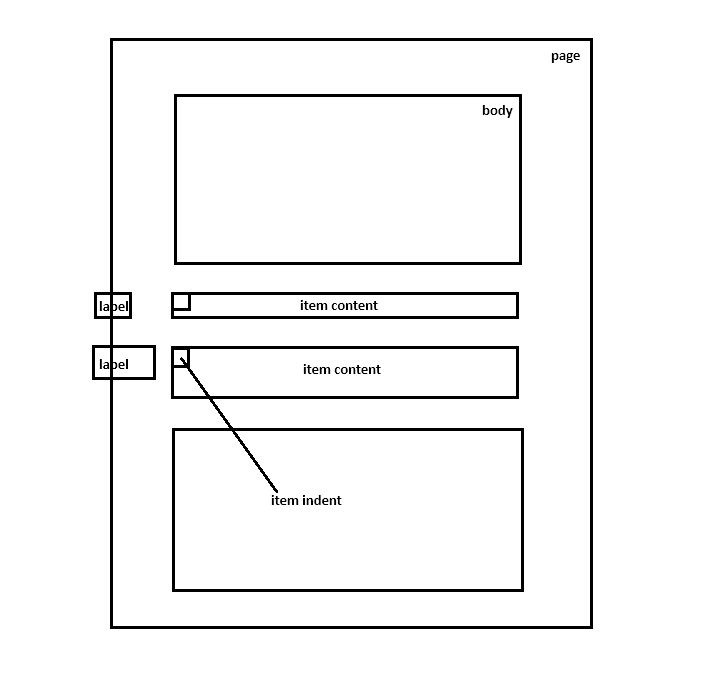
\includegraphics[width=.85\linewidth]{./list.png}
  \caption{List environment}
  \label{fig:List-env}
\end{figure}

For that is the label with is not enough, then the indent of the first line of the item will be increase.

\newenvironment{newlist}{
\begin{list}{\textbf{Newlist-\Roman{Bean}}}{
  \usecounter{Bean}
  \setlength{\leftmargin}{0pt}
  \setlength{\rightmargin}{0pt}
  \setlength{\labelwidth}{0em}
  \setlength{\labelsep}{2ex}
  \setlength{\itemindent}{2ex}
  \setlength{\parsep}{2em plus .5em minus 1.5em}
}
}{\end{list}}

\begin{newlist}
\item \text 
\item \text\setcounter{Bean}{10}
\item[\textbf{NewNewNew List-\Roman{Bean}}] \text
\end{newlist}


\subsection{trivlist}
\text
\begin{trivlist}
  \item[\textbf{Label Label Label 1}] This is the first item.
  \item[\textbf{Label Label 2}] This is the second item.
  \item No Label item content
\end{trivlist}

\section{\LaTeX{} \texttt{itemize}}
\text
\begin{itemize}
  \item[\textbf{Label Label Label 1}] This is the first item.
  \item[\textbf{Label Label 1}] This is the second item.
  \item No Label item content
  \item \text
\end{itemize}


\section{Get length}
\subsection{LaTeX method}
\begin{verbatim*}
\newlength{\mylen}
\settowidth{\mylen}{aa}
\the\mylen
\end{verbatim*}

\newlength{\mylen}
\settowidth{\mylen}{aa}
\the\mylen



\subsection{TeX primitive}
\begin{verbatim*}
\newdimen\mywidth
\setbox0=\hbox{aa}
\mywidth=\wd0
\the\mywidth
\end{verbatim*}


\newdimen\mywidth
\setbox0=\hbox{aa}
\mywidth=\wd0
\the\mywidth



\section{Tabbing environment}
In my opinion, this environment makes it easy to typeset algriothm.

\begin{tabbing}
Hello \=\kill
word \=\kill
$x$  $\leftarrow 0$ \\
while \= $x\leq 10$ do \\
      \> $x \leftarrow x+1$ \\
end while 
\end{tabbing}

That's ia to say that a \verb|\>| must has a corresponding \verb|\=| in the above line. Additionally, 
the \verb|\=| resets the logically next tab stop. \verb|\=| sets a tabulator, which can be again reached by \verb|\>|. 
\verb|\kill| cancels the line, but keeps the tabulator settings.


We can use this to generate a table.
\begin{tabbing}
Address: \= \kill
Person: \> Alice \\
Address: \> 123 Main Street \\
City: \> Springfield \\
State: \> IL \\
Zip: \> 62701
\end{tabbing}

\end{document}
